\chapter{Results}
\label{sec:results}
In this chapter, the results for the experimental setups defined in the previous chapter are discussed.
\section{Training Configurations and Architecture}
\label{sec:training config}
As with other neural network architectures, DDPM rely on a certain configuration of parameters that can influence the training results tremendously.
Through extensive testing and experimenting, the seemingly best parameters were narrowed down. 
They were used for all datasets and evaluation tests. 
\begin{table}[h!]
    \centering
    \begin{tabular}{|c c c c c |} 
         \hline
         $\beta_{min}$ & $\beta_{max}$ & $T$ & batch size & learning rate\\ [0.5ex] 
         \hline\hline
         $10^{-6}$ & 0.02 & \{200,250\} & 32 & $10^{-3}$ \\ 
         \hline
        \end{tabular}
    \caption{Parameters for training and setting up DDPMs.}
    \label{table:params}
\end{table}
The parameters depicted in table \ref{table:params} produced the most promising results. 
For the ACN dataset, a value of 250 was chosen for T, as 200 time steps were not sufficient to produce fully denoised samples.
\section{LSM results}
\label{subsec:LSM res}
After training the models we generate a set of 5000 synthetic samples that are compared against 5000 real samples from the corresponding LSM batch. 
Doing so we can compare different results for all statistical indicators and calculate averages.
\begin{figure}[!h]
    \centering
    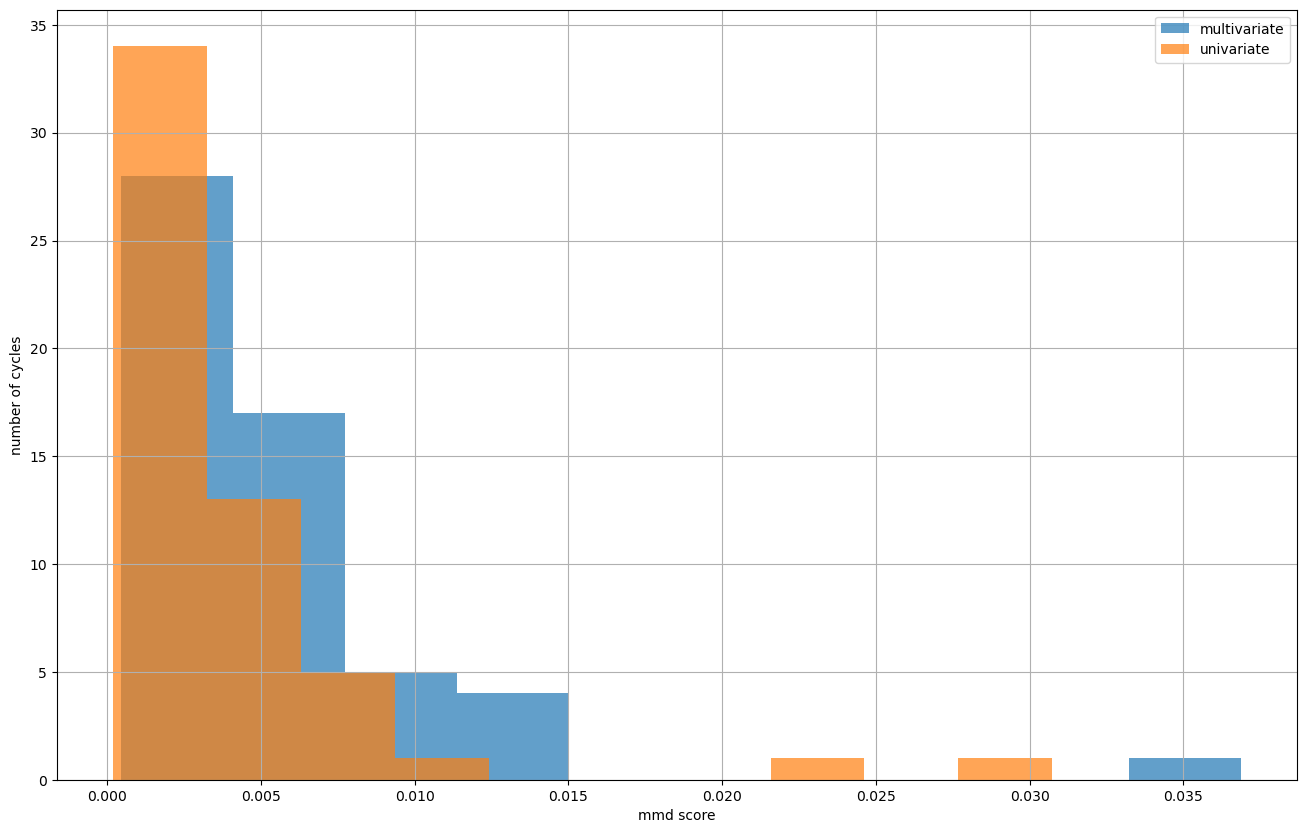
\includegraphics[width=\textwidth]{images/lsm_res_histo.png}
    \caption{Histogram of all values seen in table \ref{table:lsm results}.}
    \label{fig:lsm res histo}
\end{figure}
In Table \ref{table:lsm results}, the results for the MMD score, as described in section \ref{sec:mmd}, are presented. Both uni- and multivariate approaches yield decent results. Notably, the univariate approach, which focuses solely on synthesizing the kWhDelivered feature, demonstrates slightly better outcomes. This is evident when comparing the means, with $mean_{uni} = 0.003569$ and $mean_{multi} = 0.005349$. Additionally, a histogram of both result sets can be examined in Figure \ref{fig:lsm res histo}.\newline
In figure \ref{fig:tsne overall uni} and figure \ref{fig:tsne overall mult} t-SNE plots are depicted for all batches, as described in section \ref{sec:tsne}. Again a comparison of 5000 real and 5000 generated samples is made.
In summary, it can be concluded that the overlapping of all t-SNE plots suggests that both uni- and multivariate models performed decently.\newline
The MMD score and the t-SNE plots are used to get a statistical certainty about the quality of the data. Another venue that can be explored are visualizations that can be understood by the human eye. Therefore we look at daily means and compare them to the generated samples. Having a similar structures might be another hint for good model quality. In the following plots a comparison of characteristic days is conducted. Showing all 55 household batches is possible, but a decission was made to show only four randomly picked batches for the sake of simplicity. As seen in fig. \ref{fig:sample mean 22} the daily mean of the overall real households was picked up by the model. For more information other figures \ref{fig:sample mean 09}, \ref{fig:sample mean 37} and  \ref{fig:sample mean 53} can be seen under the Appendix section.
\begin{figure}
    \centering
    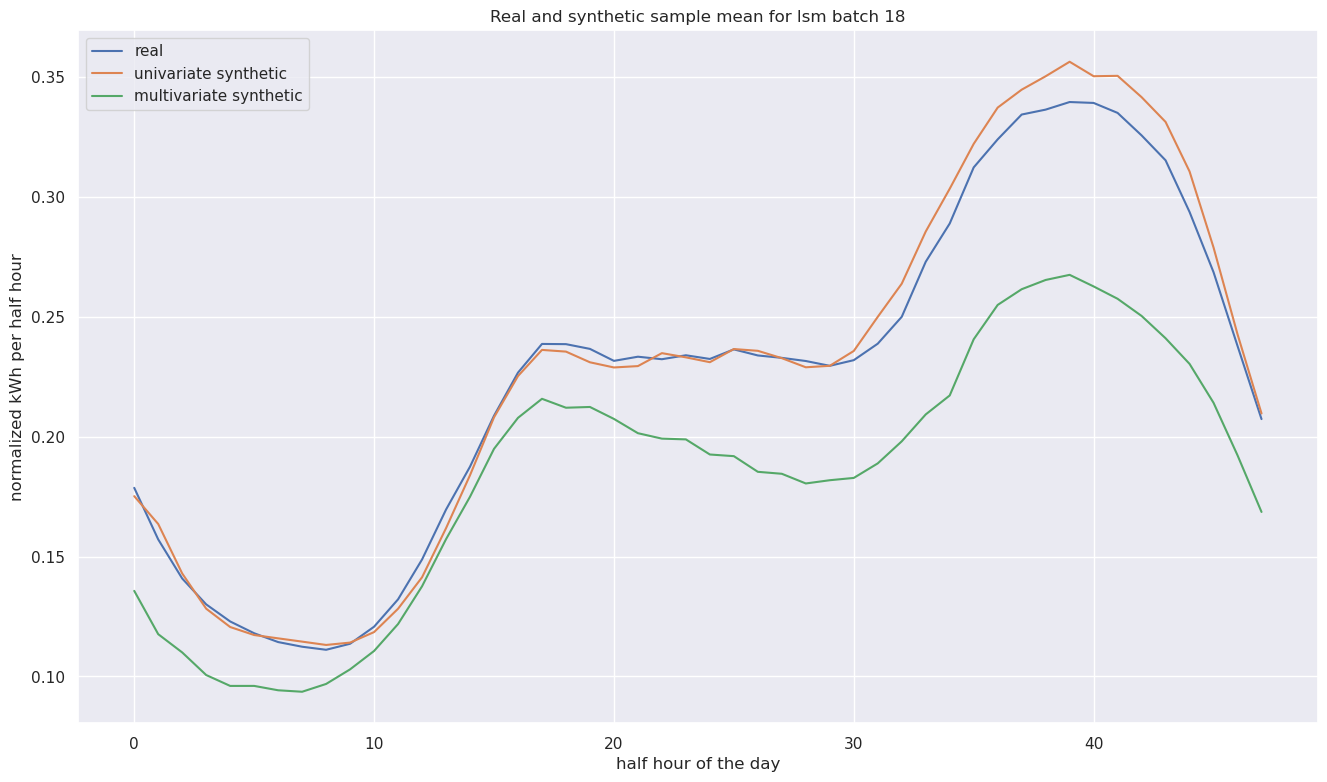
\includegraphics[width=\textwidth]{images/lsm_dm_18.png}
    \caption{Real and generated sample daily mean for lsm batch 18}
    \label{fig:sample mean 22}
\end{figure}

\section{Openmeter results}
\label{subsec:OM res}
After training, 5000 synthetic samples and 5000 randomly selected real samples were sampled to perform MMD scoring and t-SNE plots. Additionally, daily mean plots comparing real and synthetic data are presented in Figure \ref{fig:om dm}. Although differences are noticeable between all three graphs, the overall trend of the data was captured accurately. The MMD scores can be seen in Table \ref{table:om results}.
\begin{figure}
    \centering
    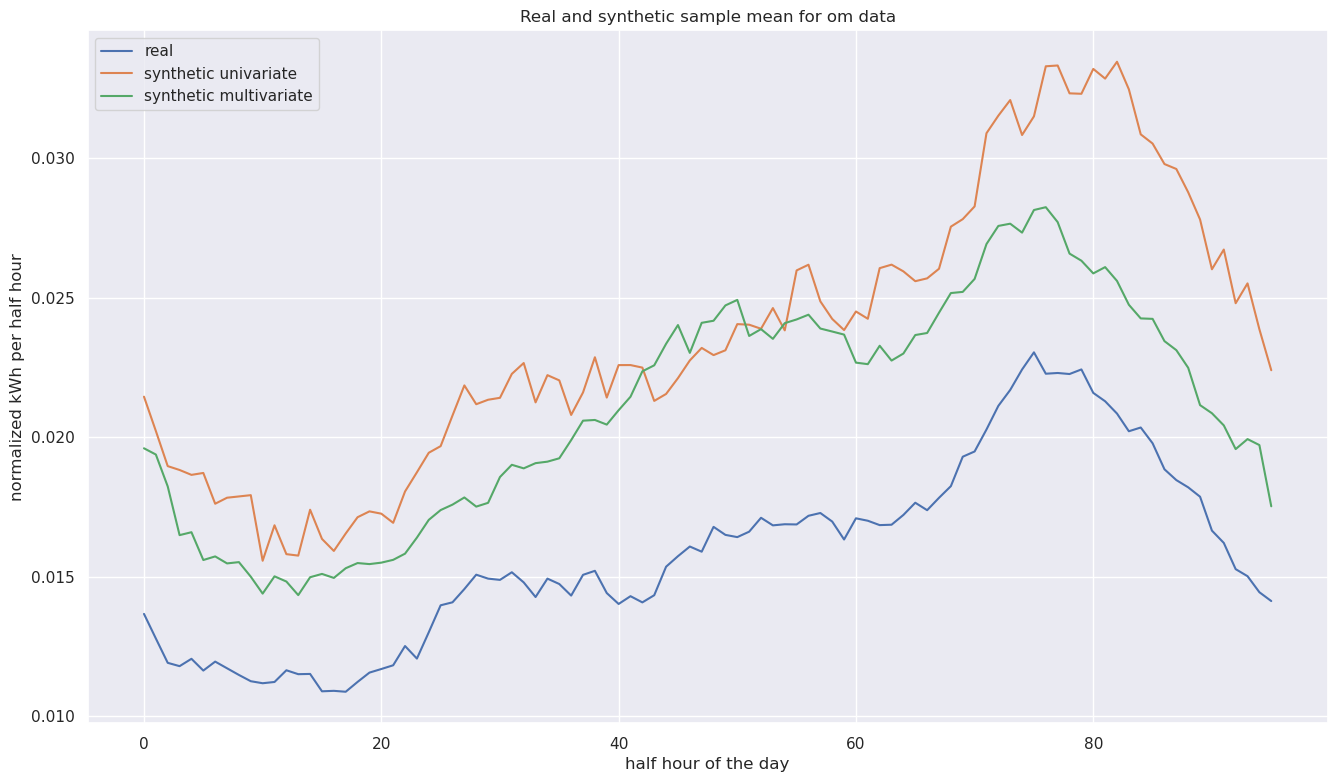
\includegraphics[width=\textwidth]{images/om_dm_private.png}
    \caption{Real and generated sample daily mean for om private data}
    \label{fig:om dm}
\end{figure}
\begin{table}[h!]
    \centering
    \begin{tabular}{|c | c c|}
        \hline
         & univariate & multivariate\\
        \hline\hline
        mmd score & 0.033825 & 0.074251\\
        \hline
    \end{tabular}
    \caption{Results for the uni-/multivariate openmeter experiments.}
    \label{table:om results}
\end{table}
The t-SNE plots can be examined in figures \ref{fig:om tsne multi} and \ref{fig:om tsne uni}. The mmd-scores suggest that the multivariate approach performed worse. The t-SNE on the other hand doesn't suggest a clear successor. Overall it can be argued that the complexity of synthesizing more features can have a negative impact on the overall quality but further experiments need to be performed to verify or falsify this assumption.
Multivariate models are non the less better due to the fact that they produce a spectrum of targets which is more likely for a real world scenario where many different time series are useful.
\section{ACN results}
\label{subsec:ACN res}
In the combined plots seen in figures \ref{fig:all acn} all daily means of the different channels can be seen. They are reconstructed almost identically.
\begin{figure}
\begin{subfigure}{.45\textwidth}
  \centering
  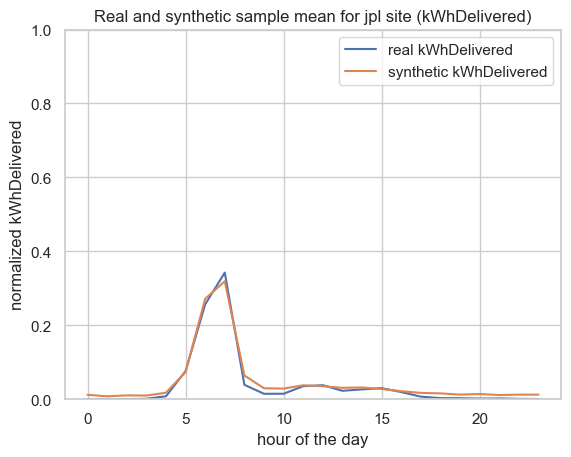
\includegraphics[width=.8\linewidth]{images/jpl_day_mean_kwh.png}
  \caption{Real and synthetic daily mean for kWhDelivered.}
  \label{fig:kwh}
\end{subfigure}
\hfill
\begin{subfigure}{.45\textwidth}
  \centering
  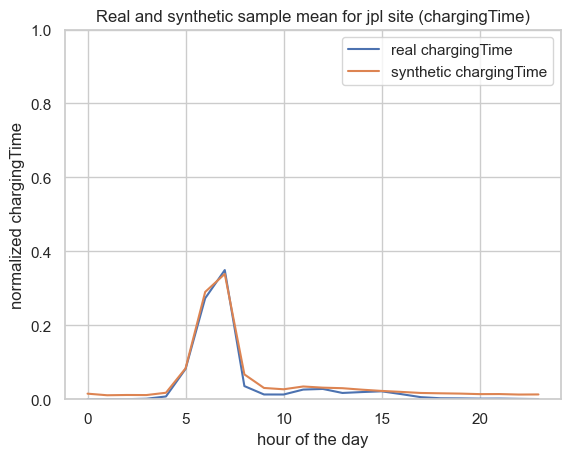
\includegraphics[width=.8\linewidth]{images/jpl_day_mean_ct.png}
  \caption{Real and synthetic daily mean for chargingTime.}
  \label{fig:ct}
\end{subfigure}
\begin{subfigure}{.45\textwidth}
  \centering
  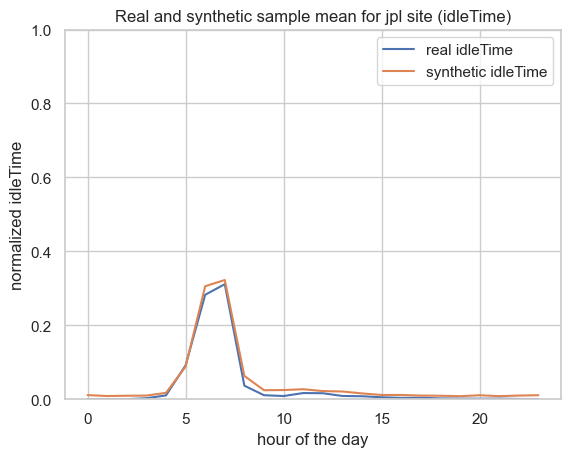
\includegraphics[width=.8\linewidth]{images/jpl_day_mean_it.png}
  \caption{Real and synthetic daily mean for idleTime.}
  \label{fig:kwh}
\end{subfigure}
\hfill
\begin{subfigure}{.45\textwidth}
  \centering
  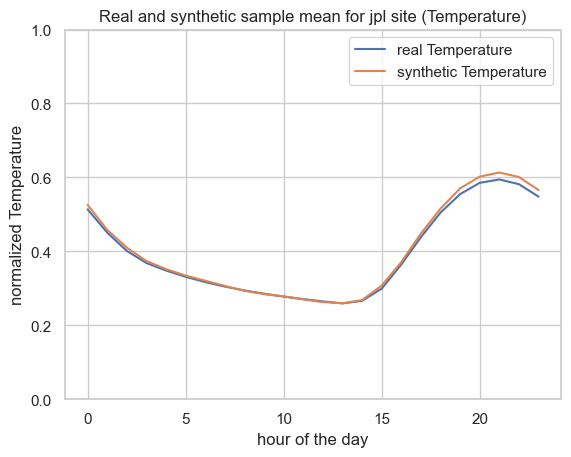
\includegraphics[width=.8\linewidth]{images/jpl_day_mean_temp.png}
  \caption{Real and synthetic daily mean for temperature.}
  \label{fig:ct}
\end{subfigure}
\begin{subfigure}{.45\textwidth}
  \centering
  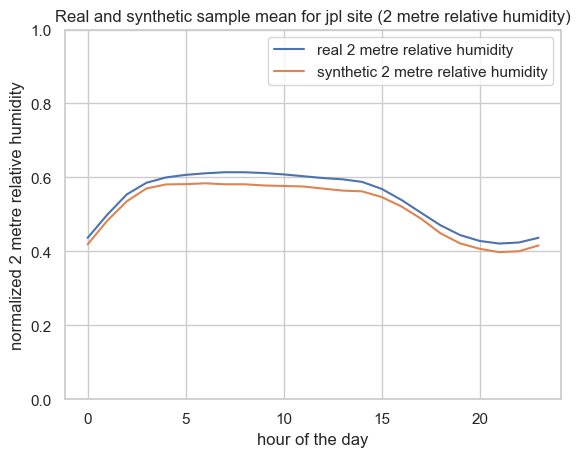
\includegraphics[width=.8\linewidth]{images/jpl_day_mean_rhum.png}
  \caption{Real and synthetic daily mean for relative humidity.}
  \label{fig:kwh}
\end{subfigure}
\hfill
\begin{subfigure}{.45\textwidth}
  \centering
  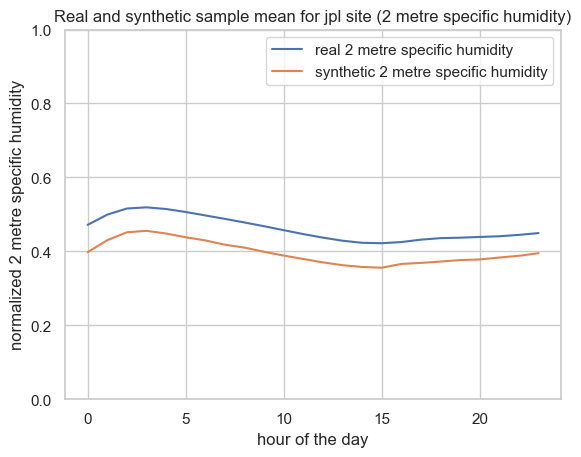
\includegraphics[width=.8\linewidth]{images/jpl_day_mean_shum.png}
  \caption{Real and synthetic daily mean for specific humidity.}
  \label{fig:ct}
\end{subfigure}
\caption{Real and synthetic daily mean for all multivariate time series features.}
\label{fig:all acn}
\end{figure}

\begin{table}[h!]
    \centering
    \begin{tabular}{|c | c  |}
        \hline
         &mmd score\\
        \hline\hline
         kWhDelivered&0.014720\\
         chargingTime&0.016854\\
         idleTime&0.008288\\ 
         Temperature&0.003077\\
         relative humidity&0.014960\\
         specific humidity&0.029262 \\
        \hline
    \end{tabular}
    \caption{Results for the multivariate ACN experiments.}
    \label{table:om results}
\end{table}%
Generally the overall data richness of the ACN dataset was significantly smaller in comparison to the LSM and OpenMeter dataset. In the end only around 500 real samples to 500 synthetic ones are compared. In the other experiments 5000 for each group were compared. This is especially important when looking at the visualization through t-SNE. Obviously the significance of those results shrinks with less samples but can still be taken into consideration. In figure \ref{fig:tsne jpl} very good results for the synthetic jpl samples can be seen.
\begin{figure}[h!]
    \centering
    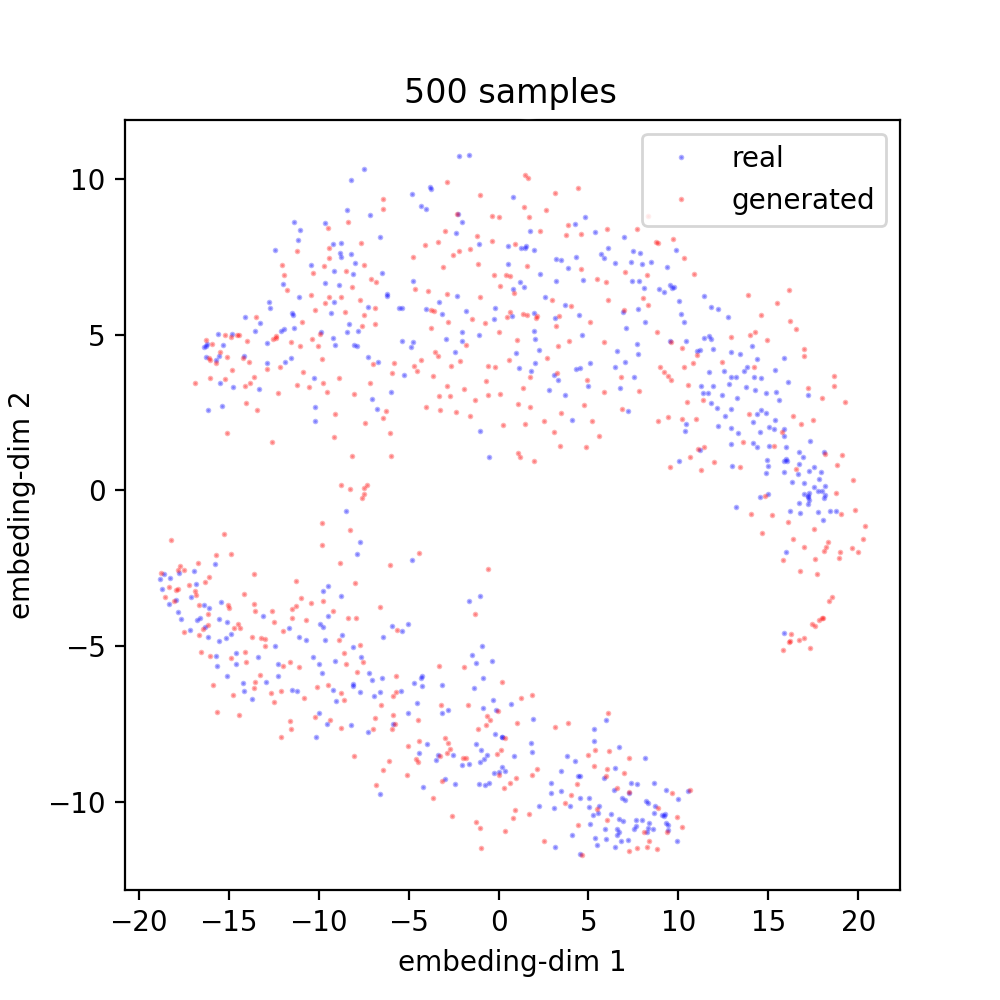
\includegraphics[width=0.6\textwidth]{images/jpl_tsne_res.png}
    \caption{t-SNE plot for 500 real and synthetic jpl site samples.}
    \label{fig:tsne jpl}
\end{figure}\newline \noindent
Finally, a look at a year of real and synthetic jpl site samples was made. A synthetic jpl site year with its rolling mean for one week is depicted in figure \ref{fig: jpl syntethic year}.
\begin{figure}[h!]
    \centering
    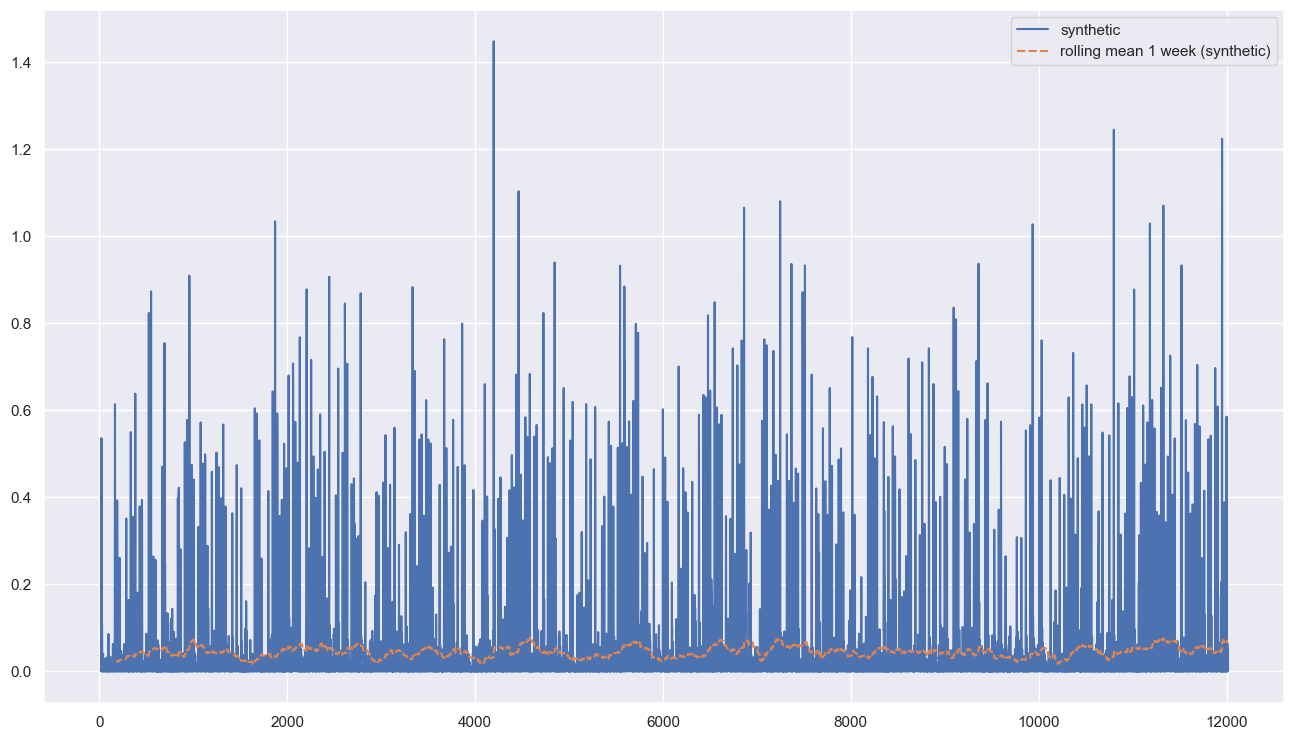
\includegraphics[width=\textwidth]{images/one_year_rm_jpl_synth.png}
    \caption{One year synthetic jpl site samples with rolling mean for one week (kWhDelivered).}
    \label{fig: jpl syntethic year}
\end{figure}\newline \noindent
Afterwards, the rolling mean for one week of one year real samples was taken and compared to the synthetic rolling mean for one week seen in figure \ref{fig: jpl year comp}.
\begin{figure}[h!]
    \centering
    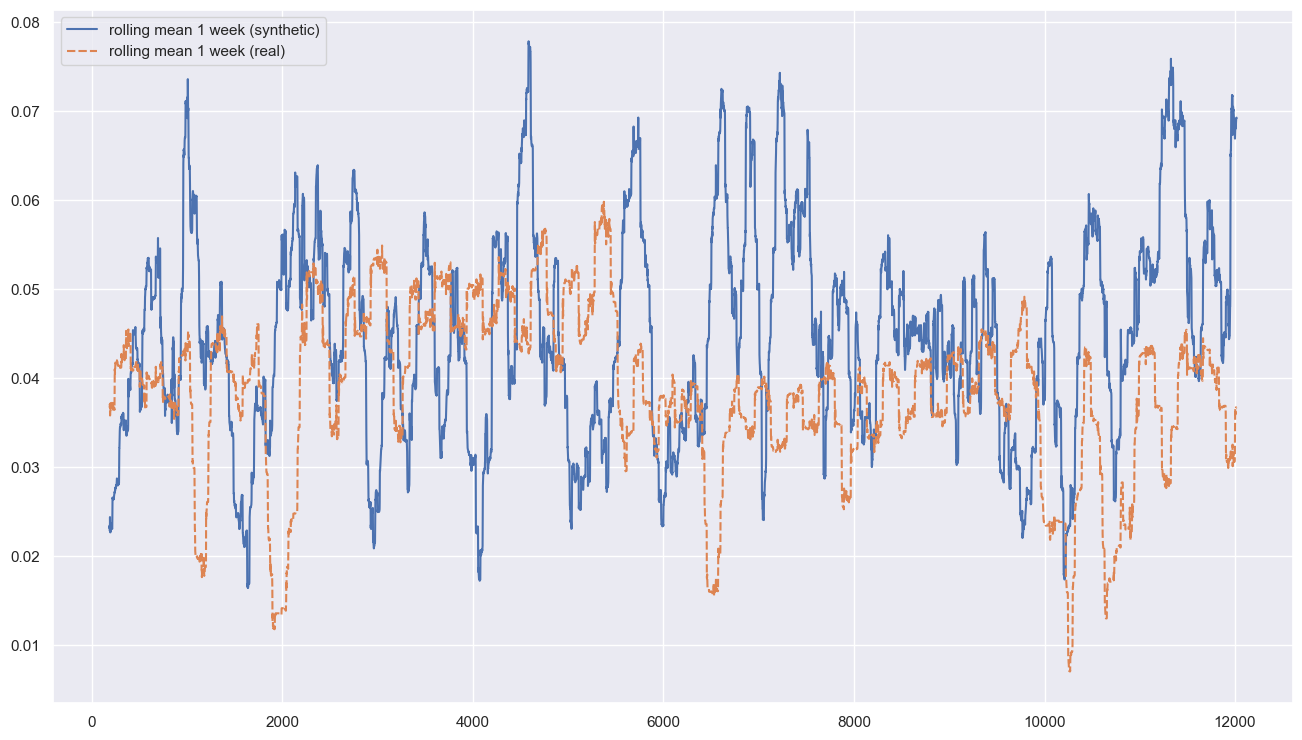
\includegraphics[width=\textwidth]{images/one_year_rm_jpl_1week_comp.png}
    \caption{One year synthetic jpl site rolling mean for one week compared to real jpl site year.}
    \label{fig: jpl year comp}
\end{figure}\newline \noindent
Overall the results look similar but on closer examination it is visible that differences especially for the comparison in figure \ref{fig: jpl year comp} occur.
The differences are small, ranging in the interval of +/- 0.04.\newline
Ultimatly, a discussion about the applicative test, that was defined in section \ref{sec:experiments} is presented. Only the results for EWC regularization terms are presented for the sake of simplicity, since all regularization terms performed similar. Looking at the following to figures \ref{fig:real forecast} and \ref{fig:synth forecast} both real and synthetic samples are shown and both were able to retain the continual learning task by still forecasting previous sections after going thru new training cycles for later sections. This similar behaviour of synthtetic and real data samples might suggest a good quality of the synthetic samples. Important to mention is that the plots do not cover four months as described when looking at the x-axis. The plots contain test samples after train/test splitting the four month datasets that make up the three sections.
\begin{figure}[h!]
    \centering
    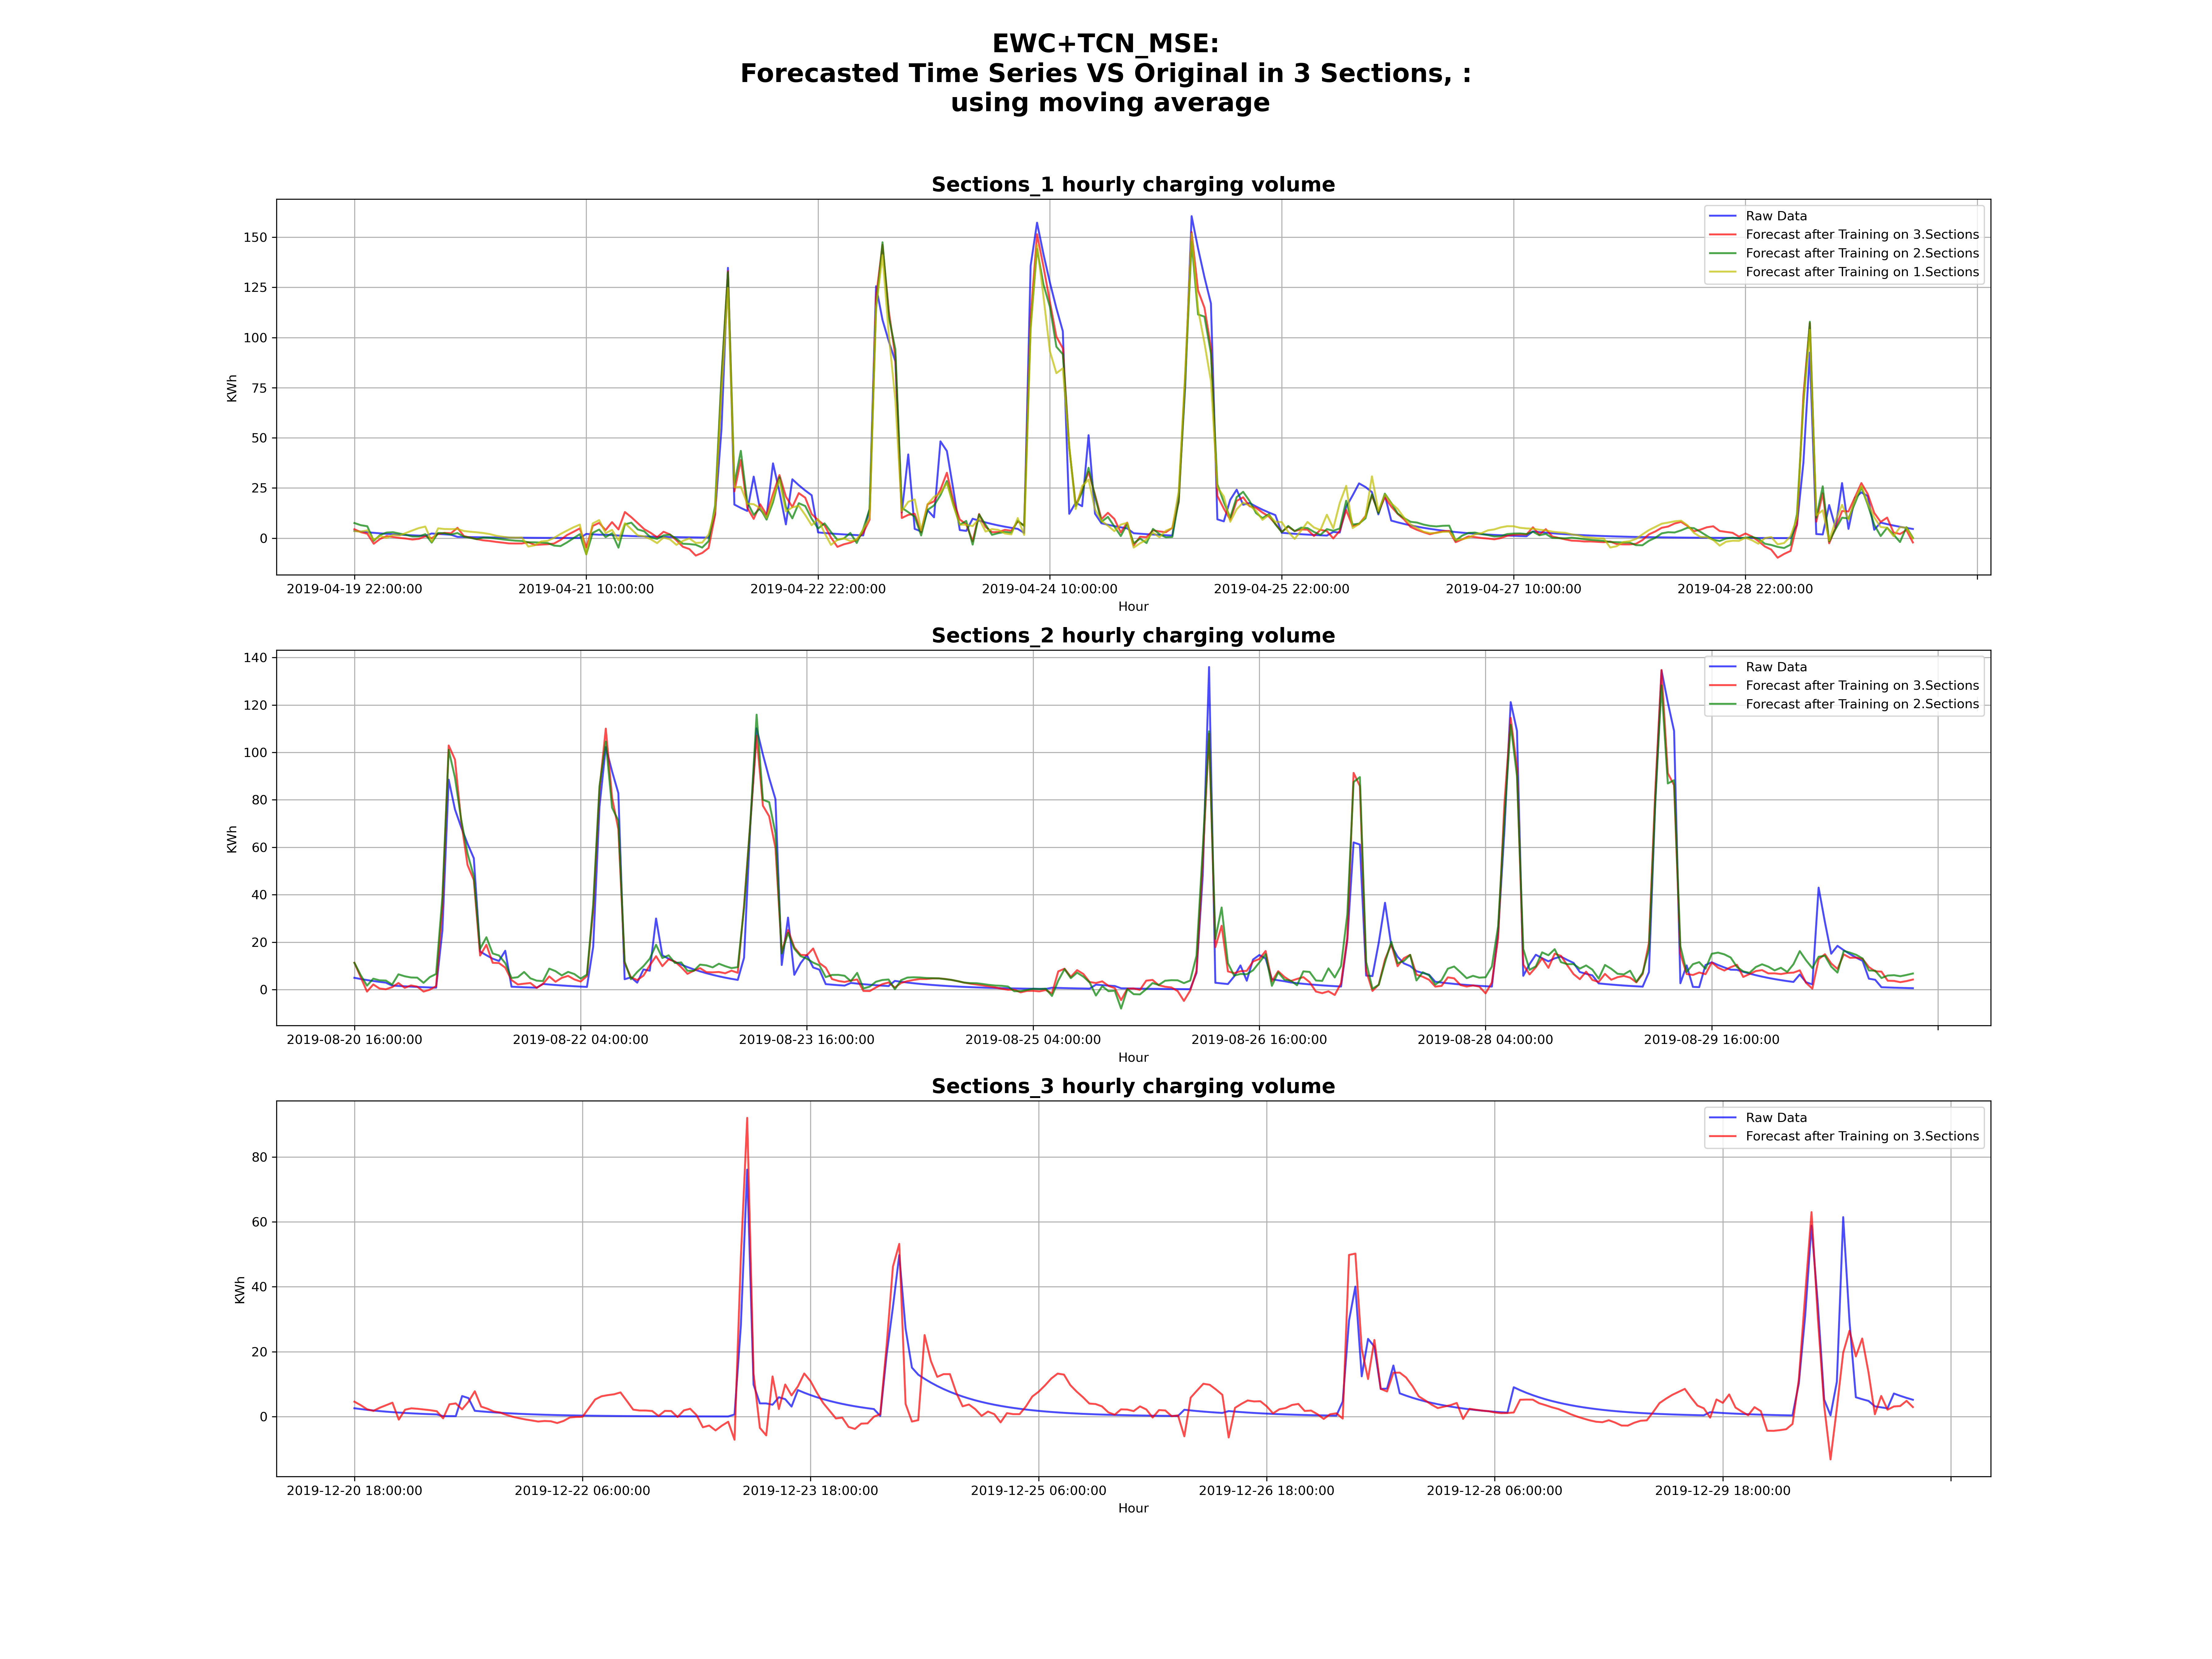
\includegraphics[width=.8\textwidth]{images/synthetic_real.png}
    \caption{CL experiment for real data jpl site samples (created by Yuan Wang).}
    \label{fig:real forecast}
\end{figure}
\begin{figure}[h!]
    \centering
    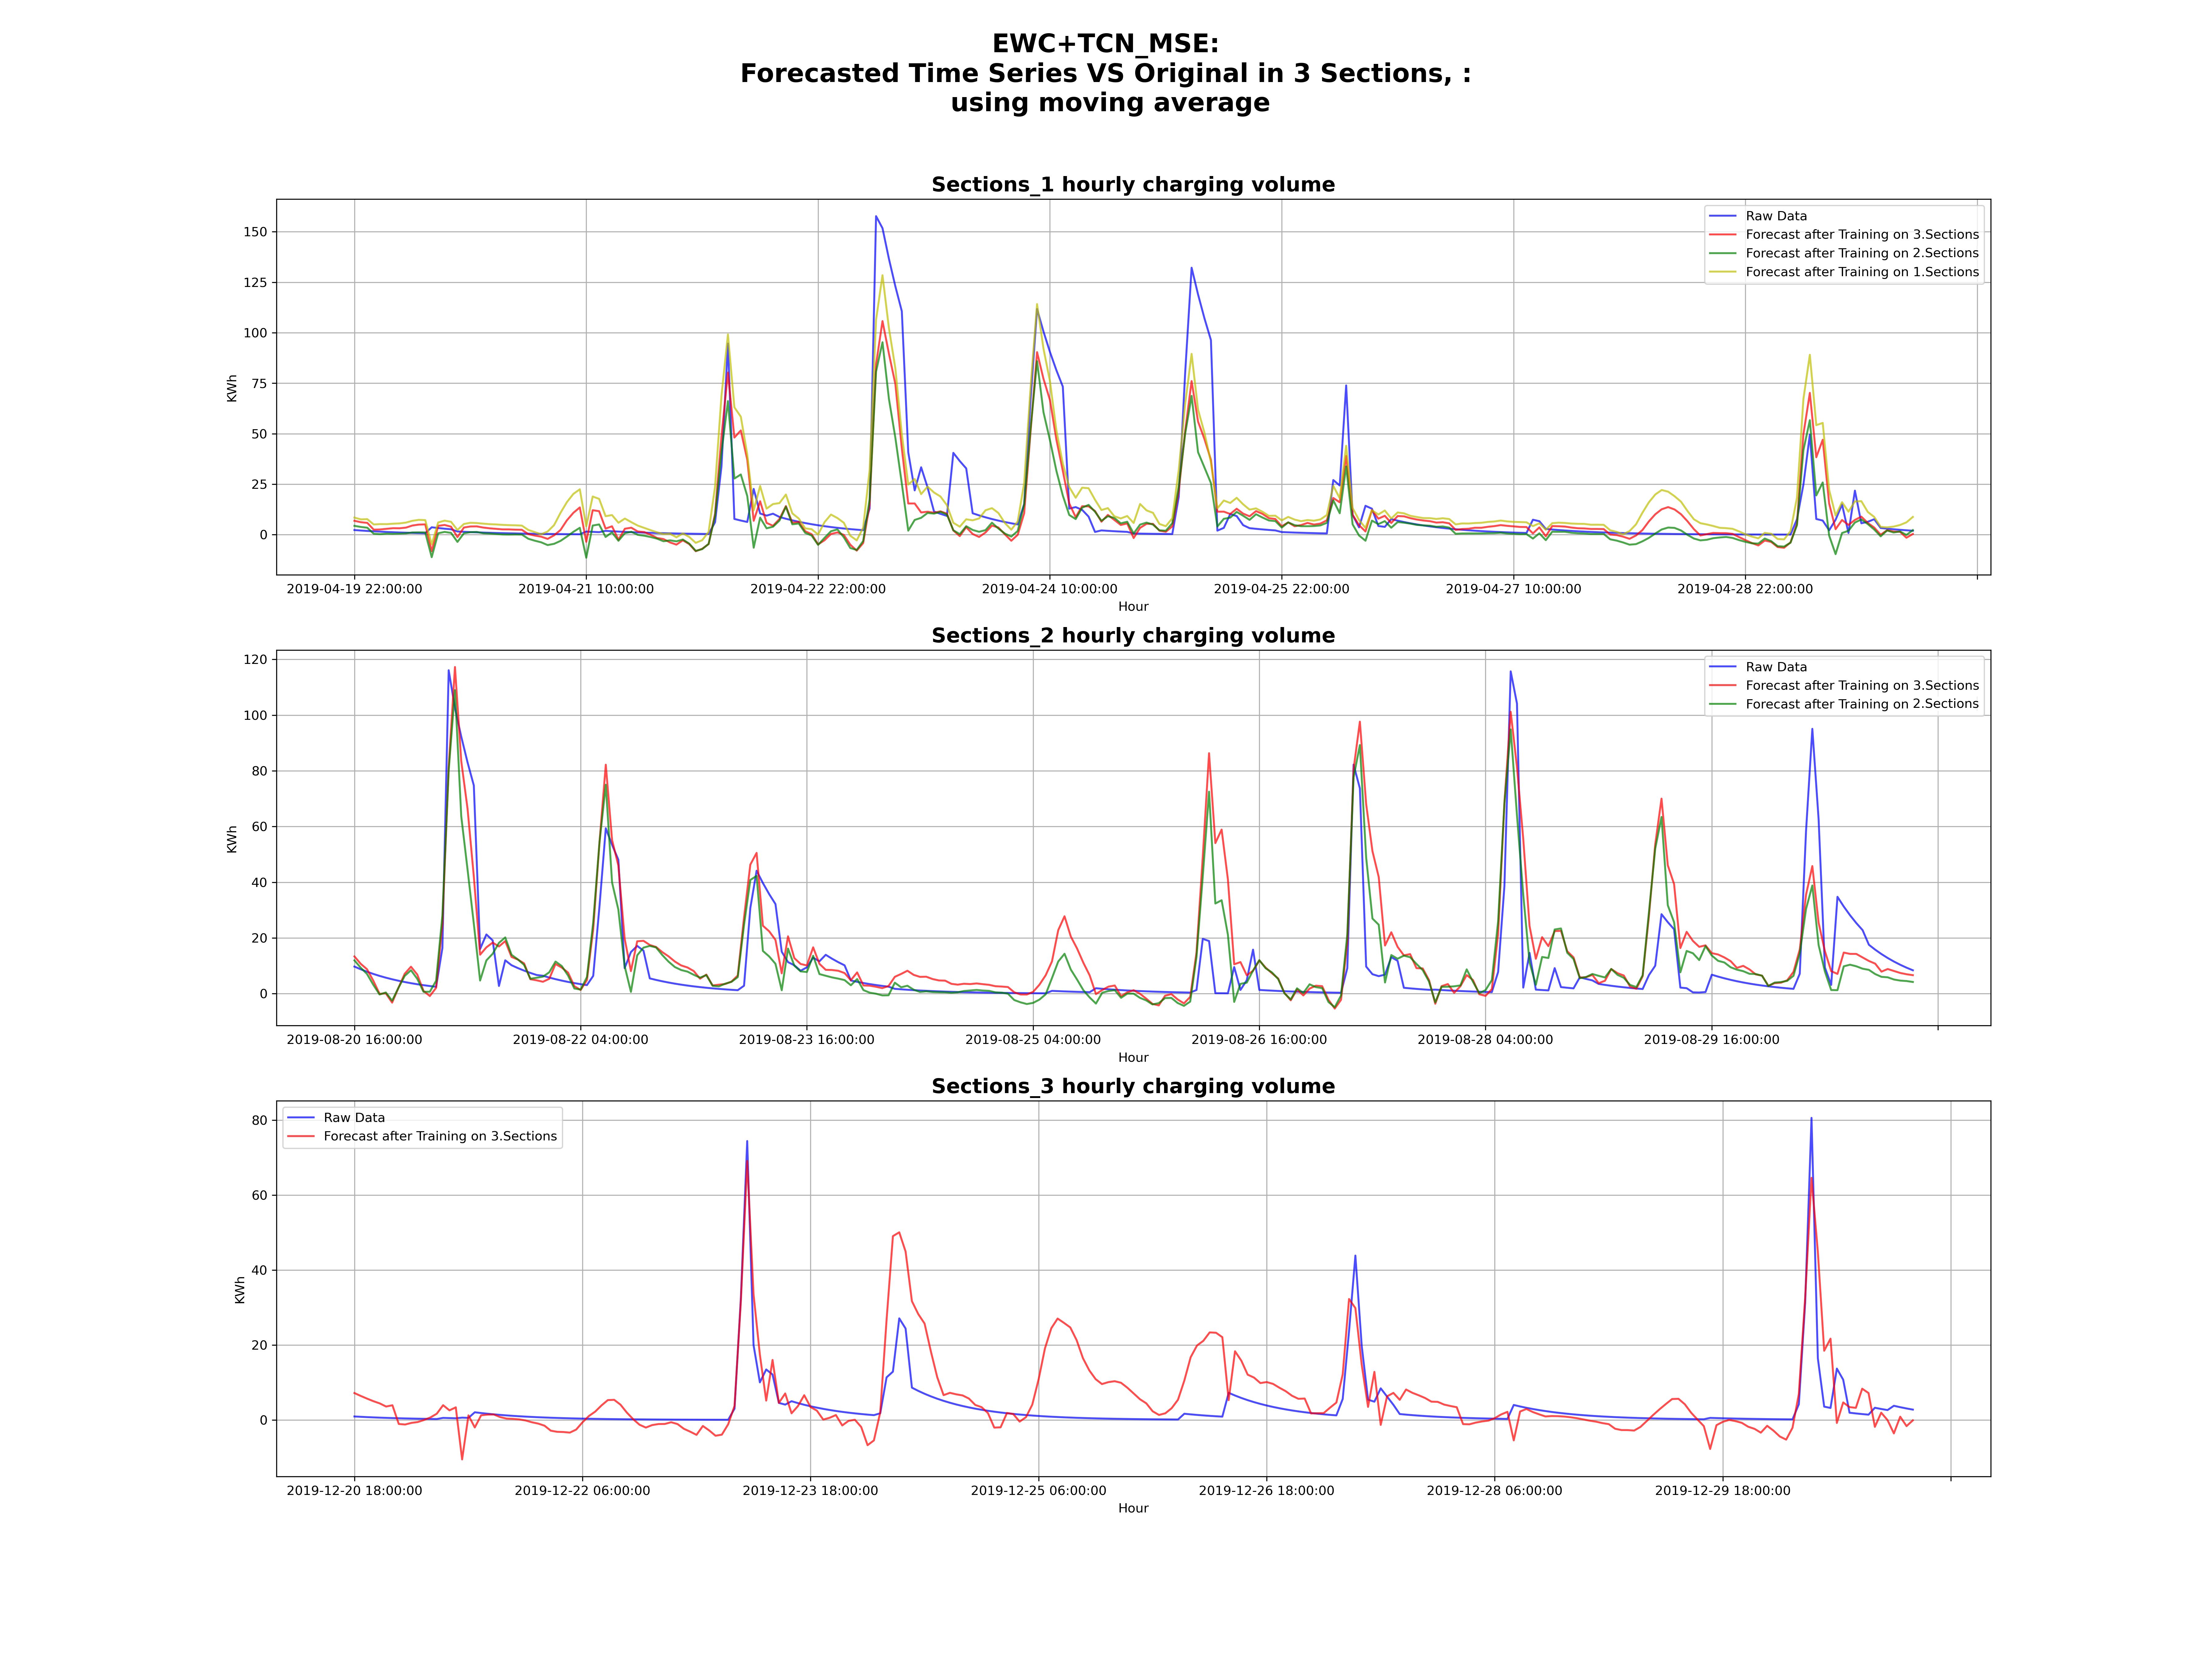
\includegraphics[width=.8\textwidth]{images/synthetic_forecast.png}
    \caption{CL experiment for synthetic data jpl site samples (created by Yuan Wang).}
    \label{fig:synth forecast}
\end{figure}